\documentclass[11pt]{scrartcl}
\usepackage[parfill]{parskip}
\usepackage{graphicx}
\usepackage{booktabs}
\usepackage{tabulary}
\usepackage{float}
\usepackage{eurosym}
\usepackage{hyperref}

\graphicspath{{../images/}}

\title{\textbf{Project Management}}
\subtitle{Apache Software Foundation}
\author{Ricardo Garc\'ia Fern\'andez}
\date{\today}

\begin{document}

\maketitle

\vfill

\begin{flushright}
    \copyright  2013 Ricardo Garc\'ia Fern\'andez - ricardogarfe [at] gmail [dot] com.

    This work is licensed under a Creative Commons 3.0 Unported License.
    To view a copy of this license visit:
 
    \url{http://creativecommons.org/licenses/by/3.0/legalcode}.
\end{flushright}

\begin{figure}[h]
    \begin{flushright}	
        
\includegraphics{by}
        \label{fig:by}
    \end{flushright}
\end{figure}

\newpage

\section{Introduction}

\emph{Apache Software Foundation}: ASF. \textbf{501.3 epigrafe C Fundación sin ánimo de lucro}

\par Un paraguas legal que nos permita la legalidad aportando transparencia.

\par Creación de un servidor web para generar los proveedores.

\par Se crea la fundación para la protección, respaldo frente a empresas, aceptar donaciones legalmente, manejar recursos. Aisla a los voluntarios de los ataques legales por parte de clientes. Defensa de marca. No más de la mitad del dinero puede venir de una sola empresa.

\section{Meritocracy}
\label{sec:meritocracy}

\par Programadores, Documentalistas, Traductores\ldots

\par ¿ Como se valoran las contribuciones ? Responder dudas a través del irc, correos, esta parte es importante por la parte de gestión de voluntarios.

\par El éxito de un proyecto radica en el camino de entrada.

\par Por otra parte, también se utiliza la conocida 'do-cracy'. Derecho en el código a desarrollar una solución comparable para poder exponerla a la comunidad.

\par No se puede esperar que una comunidad de FLOSS trabaje de la misma forma que un proyecto de una empresa privada. Objetivos y personas frente a personas y objetivos.

% section meritocracy (end)

\section{Respeto}
\label{sec:respeto}

Diversidad, mejor tratamiento a las personas al ser un proyecto global, género, culturas, etc\ldots, evitando la balcanización de proyectos.

% section respeto (end)

\section{Evolutive Software}
\label{sec:evo-software}

\par Los proyectos FLOSS se clasifican como software evolutivo interno, de la comunidad. Se ha de tener claro donde se encuentra el proceso de desarrollo del proyecto, es muy important saber el estado en el que se encuentra.

% section evo-software (end)

\section{Cadena de mérito}
\label{sec:merit-chain}

\par Las fases, roles de usuario para un proyecto dentro de la comunidad Apache se clasifican en:
\begin{itemize}
	\item Usuario.
	\item Committer.
	\item Miembro del proyecto.
	\item Miembro de la fundación ASF.
\end{itemize}

\par Organigrama de organización de los proyectos en la ASF:

\begin{figure}[htp]
\centering
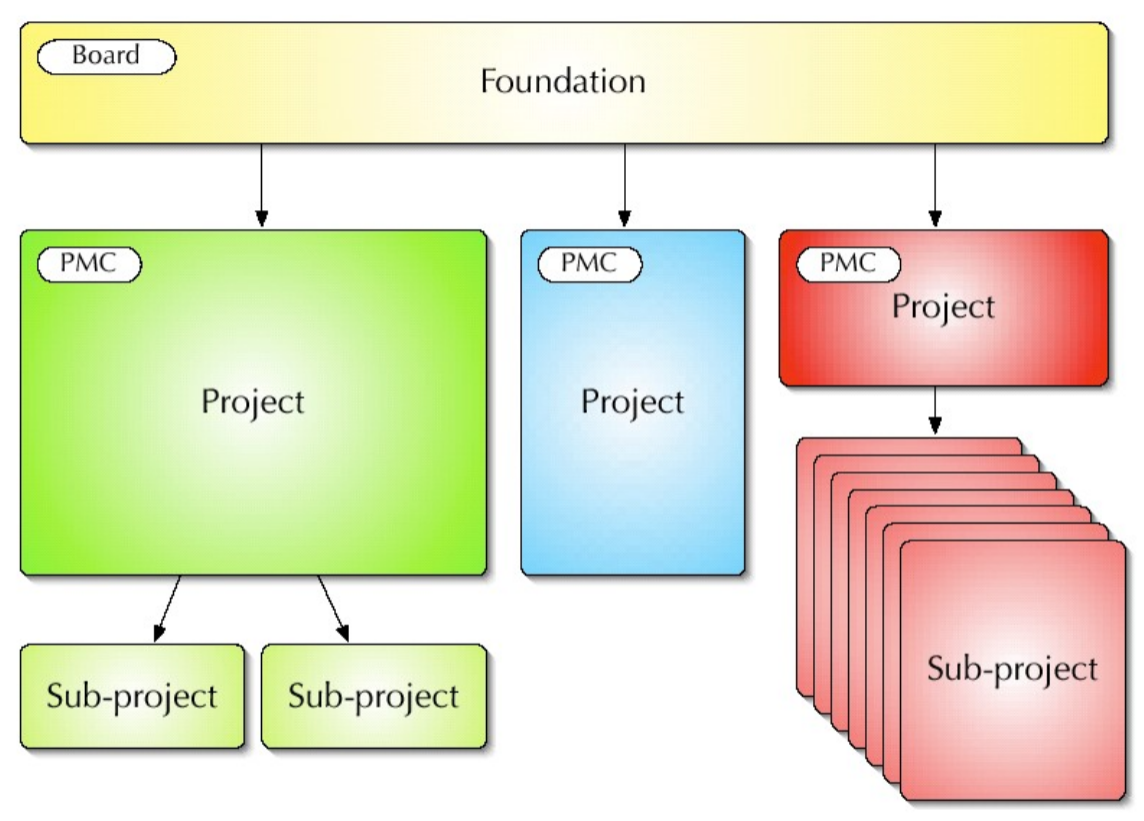
\includegraphics[width=0.7\textwidth]{asf-structure.png}
\caption{}
\label{}
\end{figure}

% section merit-chain (end)

\section{Toma de decisiones}
\label{sec:decisiones}

\par La forma de votación que se utiliza en el board director es \emph{single transferable vote}\footnote{\url{http://en.wikipedia.org/wiki/Single_transferable_vote}}.

\par En los PMC se utilizan las listas de correo para consensuar opiniones. El correo electrónico es un canal de comunicación asíncrono que permite la comunicación alrededor del mundo sin restricciones de la hora. Por ello se dan tres días para contabilizar las votaciones.

\par Siendo medios públicos se puede obtener el histórico de la toma de decisiones y la resolución de conflictos.

\par Se utiliza el consenso perezoso, 3 positivos ninguno negativo para aceptar una petición.

\begin{itemize}
	\item \textbf{+1} - De acuerto y dispuesto a ayudar.
	\item \textbf{+0} - De acuerdo, pero no puedo ayudar.
	\item \textbf{-0} - No estoy de acuerdo, pero adelante.
	\item \textbf{-1} - veto, necesita de una explicación argumentando del porqué.
\end{itemize}

\par Si no se llega a un acuerdo claro, el precursor de veto tiene una alternativa de desarrollar la solución a parte.

% section decisiones (end)

\section{Licence}
\label{sec:licence}

\par No recíproca, anti-patentes, no es compatible con GPLv2 pero sin con GPLv3.

\par Código con menos obligaciones que Apache (BSD - receptores egoístas, dador universal), (GPL - receptor universal).

% section licence (end)

\section{Proyectos de Software}
\label{sec:software-projects}

\par Incubación del proyecto:

\par Se quería evitar que la ASF se convirtiera en un sumidero de código. Se requiere una infrastructura básica para la inclusión en la incubadora:
\begin{itemize}
	\item Base de código fuente.
	\item Derecho de usarlo con la Licencia Apache v2.0.
	\item Miembro o ejecutivo responsable.
	\item (Campeón ?)
\end{itemize}

\par El proyecto que se dona a la ASF ha de cumplir una serie de requisitos, comunidad de desarrolladores activos (3).

% section software-projects (end)

\section{Ático}
\label{sec:atico}

\par ASF tiene un apartado dedicado para los proyectos inactivos, \emph{Apache Attic}. Gestiona las listas de correo y los repositorios de código.

% section atico (end)

\section{Lab}
\label{sec:lab}

\par Paso previo a la incubación y parecido al ático. No permite liberar versiones del código para que la gente no caiga en 'la trampa' de la versión.

% section lab (end)

\section{Apache extra}
\label{sec:extra}

\par Este apartado se encarga de hospedar los proyectos relacionados indirectamente con otros de Apache, es decir, utilizando herramientas o librerías ampliando funcionalidades, etc\ldots

% section  (end)
\end{document}
